\documentclass[smaller]{beamer} % Frame size:  128mmx96mm
% smaller:  beamer font size
% draft:    graphicx mode

%\usepackage[draft]{graphicx}
\usepackage[normalem]{ulem}     % for \sout
\usepackage[percent]{overpic}   % for \overpic
\usepackage{anyfontsize}        % for huge "X"

\mode<presentation>
{
    \usetheme{Berkeley}
}

\logo{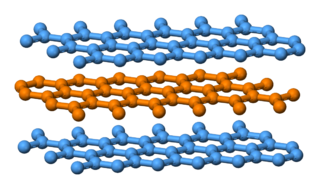
\includegraphics[height=10mm]{img/Graphite.png}}
\begin{document}

\setbeamerfont{tinyfont}{size=\tiny}
\setbeamerfont{smallfont}{size=\small}

\section{Graphite}
\begin{frame}{Graphite}
    \begin{tabular}{l}
        Kurt Starsinic {\tt $<$kstarsinic@gmail.com$>$} \\
        {\tt http://github.com/kstarsinic/presentations/} \\ % XXX create
        {\tt http://www.cpan.org/authors/id/K/KS/KSTAR/} \\
        \\
        Philadelphia Perl Mongers \\
        November 5, 2012 \\
    \end{tabular}
\end{frame}

\subsection{no, not {\it that} graphite}
\begin{frame}{Graphite}{no, not {\it that} graphite}
    \begin{tabular}{|l|l|}
        \hline
        \sout{Graphite}     & {\tt http://graphite.sil.org/}  \\
        \ \sout{(SIL)}      &                           \\ \hline

        \sout{Alice}        & {\tt http://alice.loria.fr/} \\
        \ \sout{Graphite}   & {\tt \ WIKI/index.php/Graphite/Graphite} \\ \hline

        \sout{Graphite}     & {\tt http://www.ashlar.com/} \\
        \ \sout{CAD}        & {\tt \ 2d-3d-drafting/2d-3d-cad-graphite.html} \\ \hline

        Graphite            & {\tt http://graphite.wikidot.com/} \\
        \ Scalable          & \\
        \ Realtime          & \\
        \ Graphing!         & \\ \hline
    \end{tabular}
\end{frame}

\section{What is Graphite?}
\begin{frame}[fragile]{What is Graphite?}
    A timeseries data dashboard
    \vskip10pt
    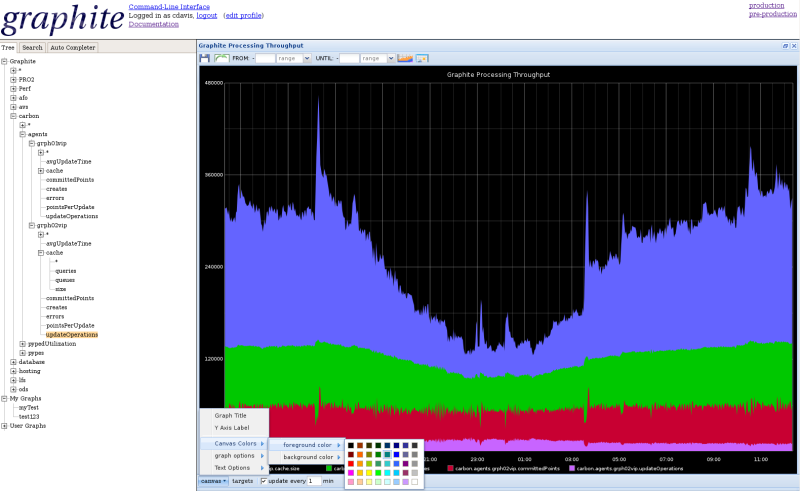
\includegraphics[width=0.9\textwidth,height=0.9\textheight,keepaspectratio]{img/Screenshot.png}
    \vskip10pt
    \usebeamerfont{tinyfont}
    source:  http://graphite.wdfiles.com/local--files/screen-shots/graphite\_fullscreen\_800.png
\end{frame}

\begin{frame}{What is Graphite?}
    A timeseries data dashboard
    \vskip10pt

    Functions:
    \begin{itemize}
        \item Web application framework
        \item Numeric timeseries round robin database
        \item Graphing and rendering engine
    \end{itemize}

    \vskip10pt
    Components:
    \begin{itemize}
        \item graphite-web
        \item carbon
        \item whisper
    \end{itemize}
\end{frame}

\begin{frame}[fragile]{What is Graphite?}
    \begin{columns}[T]
        \begin{column}{.5\textwidth}
            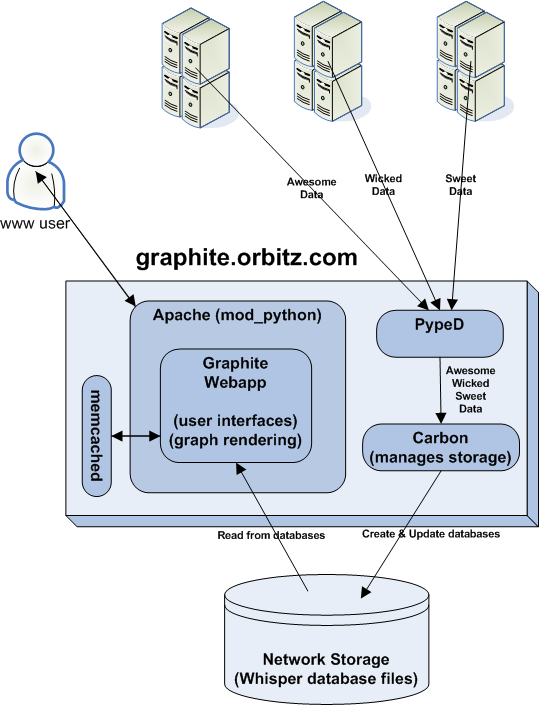
\includegraphics[height=60mm]{img/GHL.png}
        \end{column}
        \begin{column}{.5\textwidth}
            \uncover<2->{
                Legend:
                \begin{itemize}
                    \item apache/graphite (web app)
                    \item carbon (storage manager)
                    \item whisper (round robin database)
                \end{itemize}
            }

            \uncover<3->{
                \vskip10pt
                Myth:
                \begin{itemize}
                    \item Use {\tt mod\_wsgi}, {\it not} {\tt mod\_python}
                    \item {\tt PypeD} isn't necessary, and isn't exciting
                    \item {\tt memcached} is optional
                \end{itemize}
            }
        \end{column}
    \end{columns}

    \vskip10pt
    \usebeamerfont{tinyfont}
    source: http://graphite.wikidot.com/local--files/high-level-diagram/Graphite\%20High\%20Level.png
\end{frame}

\begin{frame}[fragile]{What is Graphite?}
    \begin{columns}[T]
        \begin{column}{.5\textwidth}
            \begin{overpic}[height=60mm]{img/GHL.png}
                \put (5,10) {\fontsize{190}{190}\selectfont X}
            \end{overpic}
        \end{column}
        \begin{column}{.5\textwidth}
            Legend:
            \begin{itemize}
                \item apache/graphite (web app)
                \item carbon (storage manager)
                \item whisper (round robin database)
            \end{itemize}

            \vskip10pt
            Myth:
            \begin{itemize}
                \item Use {\tt mod\_wsgi}, {\it not} {\tt mod\_python}
                \item {\tt PypeD} isn't necessary, and isn't exciting
                \item {\tt memcached} is optional
            \end{itemize}
        \end{column}
    \end{columns}

    \vskip10pt
    \usebeamerfont{tinyfont}
    source: http://graphite.wikidot.com/local--files/high-level-diagram/Graphite\%20High\%20Level.png
\end{frame}

\subsection{What is Graphite \it{not?}}
\begin{frame}{What is Graphite \it{not?}}
    \begin{itemize}
        \item A general-purpose database
        \item A general-purpose graphing toolkit
        \item Written in Perl
    \end{itemize}
\end{frame}

\section{Component}
\subsection{Graphite}
\begin{frame}[fragile]{Graphite}
    \begin{itemize}
        \item Web app: \\
        {\tt \ \ http://graphite.wikidot.com/url-api-reference}
        \item Command line: \\
        {\tt \ \ http://graphite.wikidot.com/cli-reference}
    \end{itemize}
\end{frame}

\subsection{Carbon}
\begin{frame}[fragile]{Carbon}
    \def\filler{\tt\ \ \ \ \ \ \ \ \ \ \ \ \ \ \ \ \hfill}
    \def\qafiller{\tt\ \ \ \ \ \ \ \ \ \ \ \ \ \ \hfill}
    \begin{description}
        \item<1->[\tt carbon-agent\ \ \ \ \hfill]       Master process (starts others)
        \item<1->[\filler]                              Listens on a port (default 2003) for inserts
        \item<1->[\filler]                              Simple syntax:
        \item<1->[\filler]                              \verb|  printf SOCKET "%s %f %d",|
        \item<1->[\filler]                              \verb|         $path, $value, $time|
        \item<2->[\tt carbon-cache\ \ \ \ \hfill]       Receives updates from carbon-agent, aggregates
        \item<2->[\filler]                              them, writes them to carbon-persister
        \item<2->[\filler]                              as quickly as possible
        \item<3->[\tt carbon-persister\hfill]           Writes updates to disk via whisper API
        \item<4->[Q:\qafiller]                      Why so many moving parts?
        \item<5->[A:\qafiller]                      Because python's ``threading'' model isn't.
    \end{description}

    \uncover<5->{
        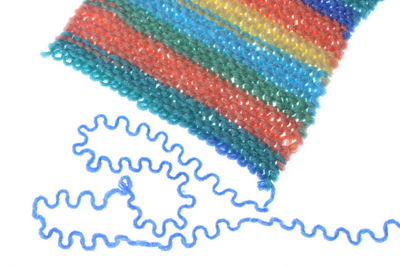
\includegraphics{img/Unravel400.jpg}
        \usebeamerfont{tinyfont}
        source:  http://www.shutterstock.com/ \hfill
    }
\end{frame}

\subsection{Whisper}
\begin{frame}
    Whisper

    \begin{itemize}
        \item Similar to rrd, but . . .
        \item Allows out-of-order inserts
        \item Allows irregularly-spaced inserts
        \item Allows bulk inserts
        \item {\tt http://graphite.wikidot.com/whisper}
    \end{itemize}
\end{frame}

\section{Setting up Graphite}
\subsection{Components}
\begin{frame}{Setting up Graphite}{Components}
    Required:
    \begin{itemize}
        \item {\tt python} (2.4+)
        \item {\tt pycairo} (with PNG backend support)
        \item {\tt apache} with {\tt mod\_wsgi}
        \item {\tt django} (Python MVC framework for web applications) + {\tt django-tagging}
        \item {\tt twisted} (Python event management framework)
        \item {\tt sqlite3}, {\tt mysql}, {\tt postgresql}, or {\tt ado\_mssql}
    \end{itemize}

    \vskip10pt

    Optional:
    \begin{itemize}
        \item {\it python-ldap} (for LDAP-based web authentication)
        \item {\it memcached} \& {\it python-memcached} (for performance boost)
        \item {\it python-sqlite2}
        \item {\it collectd} \& {\it collectd-graphite} (to collect system stats)
    \end{itemize}
\end{frame}

\subsection{Procedure}
\begin{frame}{Setting up Graphite}{Procedure}
    Do this:
    \begin{itemize}
        \item Read:                 {\tt http://graphite.wikidot.com/installation}
        \item Apply:                {\tt https://github.com/graphite-project/carbon/pull/44}
        \item Check permissions:    {\tt /opt/graphite/storage/log/}
        \item Start apache:         {\tt apachectl start}
        \item Start carbon:         {\tt cd /opt/graphite/; python bin/carbon-cache.py start}
        \item View:                 {\tt http://localhost/}
    \end{itemize}

    \vskip10pt
    \uncover<2->{Caveats}
    \begin{itemize}
        \item<3-> Figure out file ownerships and permissions first
        \item<4-> Do {\it not} enable {\tt mod\_python}
        \item<5-> {\it Do} enable {\tt mod\_wsgi}
        \item<6-> Apply the patch!
    \end{itemize}
\end{frame}

\section{\tt\#ifdef PERL}
\begin{frame}{\tt\#ifdef PERL}
    \def\cdfiller{}
    \begin{description}
        \item[\tt collectd-graphite]
        \item[]                             {\tt https://github.com/joemiller/}
        \item[]                             {\tt \ \ \ \ \ \ \ \ collectd-graphite}
        \item[\tt collectd-perl]
        \item[]                             {\tt http://collectd.org/documentation/}
        \item[]                             {\tt \ \ \ \ \ \ \ manpages/collectd-perl.5.shtml}
        \item[\tt Net::Graphite]
        \item[]                             {\tt http://search.cpan.org/${\sim}$slanning/}
        \item[]                             {\tt \ \ \ \ \ \ \ Net-Graphite-0.10/}
    \end{description}
\end{frame}

\section{Additional References}
\begin{frame}{Additional References}
    \begin{tabular}{|l|l|}
        \hline
        Graphite            & {\tt http://graphite.wikidot.com/}                \\
                            & {\tt http://graphite.readthedocs.org/}            \\
                            & {\tt http://www.aosabook.org/en/graphite.html}    \\ \hline
        collectd            & {\tt http://collectd.org/}                        \\ \hline
        rrdtool             & {\tt http://logio.org/}                           \\ \hline

    \end{tabular}
\end{frame}

\section{Demo/Questions}
\begin{frame}{Demo/Questions}
    \begin{itemize}
        \item Demo
        \item Questions
        \item Where are we drinking?
    \end{itemize}
\end{frame}

\end{document}

